\documentclass{tufte-handout}
%------------------------------------------------
%\geometry{showframe} % display margins for debugging page layout
%------------------------------------------------
\usepackage{graphicx} % allow embedded images
  \setkeys{Gin}{width=\linewidth,totalheight=\textheight,keepaspectratio}
  \graphicspath{{/home/swl/Dropbox/ucd/eu_economics/figs/}}  % set of paths to search for images
\usepackage{amsmath}  % extended mathematics
\usepackage{booktabs} % book-quality tables
\usepackage{units}    % non-stacked fractions and better unit spacing
\usepackage{multicol} % multiple column layout facilities
\usepackage{lipsum}   % filler text
\usepackage{fancyvrb} % extended verbatim environments
  \fvset{fontsize=\normalsize}% default font size for fancy-verbatim environments

%------------------------------------------------
% Standardize command font styles and environments
\newcommand{\doccmd}[1]{\texttt{\textbackslash#1}}% command name -- adds backslash automatically
\newcommand{\docopt}[1]{\ensuremath{\langle}\textrm{\textit{#1}}\ensuremath{\rangle}}% optional command argument
\newcommand{\docarg}[1]{\textrm{\textit{#1}}}% (required) command argument
\newcommand{\docenv}[1]{\textsf{#1}}% environment name
\newcommand{\docpkg}[1]{\texttt{#1}}% package name
\newcommand{\doccls}[1]{\texttt{#1}}% document class name
\newcommand{\docclsopt}[1]{\texttt{#1}}% document class option name
\newenvironment{docspec}{\begin{quote}\noindent}{\end{quote}}% command specification environment
%------------------------------------------------

%------------------------------------------------
%%%% Details %%%%
%------------------------------------------------
\title{EU Economics: The Eurocrisis}
\author{University College Dublin}
\date{Spring 2017} 

\begin{document}
\maketitle  
%------------------------------------------------------------------------------
% THE EUROCRISIS
\section{A broad overview of the global financial crisis and the Eurozone}
A main objective of the European Union is to achieve economic convergence across the member states. 
That objective has experienced a severe setback due to the global financial crisis which lead to the sovereign debt crisis in the Eurozone. 
Let's start by examining the impact of this crisis on a range of macroeconomic indicators. 
\begin{enumerate}
  \item GDP (figure~\ref{fig:gdp})
  \begin{itemize}
    \item Countries across the EU where hit by the global recession
    \item Although this was a common shock, some countries have experienced longer lasting effects
    \item e.g. while Spain has been able to return to positive growth rates, the situation in Greece is still very dire
  \end{itemize}
  \item Unemployment (figure~\ref{fig:unemployment})
  \begin{itemize}
    \item The effect of the crisis on the unemployment rate differs per country
    \item Unemployment for the Eurozone on average went up but not by much
    \item Contrast the situation in Germany, largely unaffected, with the huge increase in Spain
  \end{itemize}
  \item Budget surplus (figure~\ref{fig:budget_surplus})
  \begin{itemize}
    \item On average the Eurozone wasn't doing that badly in terms of keeping budget close to the Maastricht Treaty guideline
    \item As a result of the crisis government budget expanded due to decrease in output
    \item Whereas Germany is relatively disciplined when it comes to budget, Greece has been running a deficit for many years
  \end{itemize}
  \item Government debt (figure~\ref{fig:public_debt})
  \begin{itemize}
    \item Whereas countries tend to adhere to the rules concerning budget deficit, levels of public debt tend to be much higher than the 60\% set by the Maastricht Treaty
    \item Even countries like Germany have been over the limit for many years, although levels are coming down in recent years compared to Eurozone average
    \item Greece's public debt levels are very high above 100\% of GDP moving towards 200\%. 
  \end{itemize}
\end{enumerate}

%--------------------------------------
% GDP
\begin{figure}
  \includegraphics[scale=.3]{crisis_gdp_growth}
  \caption{Annual GDP growth. Black line shows the average growth rate for the Eurozone, whereas the red line represents Spain and the blue line Greece. Data: Eurostat}
  \label{fig:gdp}
\end{figure}
%--------------------------------------

%--------------------------------------
% UNEMPLOYMENT
\begin{figure}
  \includegraphics[scale=.3]{crisis_unemployment}
  \caption{Unemployment rate. Black line shows the average rate for the Eurozone, whereas the red line represents Spain and the gold-coloured line Germany. Data: Eurostat}
  \label{fig:unemployment}
\end{figure}
%--------------------------------------

%--------------------------------------
% BUDGET SURPLUS
\begin{figure}
  \includegraphics[scale=.3]{crisis_budget}
  \caption{Budget surplus as percentage of GDP. Black line shows the average rate for the Eurozone, whereas the blue line represents Greece and the gold-coloured line Germany. The two black horizontal solid lines show the budget surplus allowed under the Maastricht Treaty (3\%) and a balanced budget (0\%). Data: Eurostat}
  \label{fig:budget_surplus}
\end{figure}
%--------------------------------------

%--------------------------------------
% PUBLIC DEBT
\begin{figure}
  \includegraphics[scale=.3]{crisis_gov_debt}
  \caption{Government debt as percentage of GDP. Black line shows the average rate for the Eurozone, whereas the red line represents Spain and the gold-coloured line Germany. The black horizontal line shows the allowed level of government debt under the Maastricht Treaty. Data: Eurostat}
  \label{fig:public_debt}
\end{figure}
%--------------------------------------
\clearpage

%------------------------------------------------------------------------------
\section{The Eurocrisis}
The sovereign debt crisis in the Eurozone\footnote{Which started roughly at the end of 2009} has been a particular difficult episode in EU's history. 
The crisis saw a number of countries unable to repay or refinance their sovereign debt, needing external assistance.\marginnote{For instance from other countries in the Eurozone, the EU itself, the European Central Bank, or the International Monetary Fund.} 
Countries that were particularly hard hit include\footnote{One factor contributing to the severity of the crisis in these countries was the limited buffer to conduct countercyclical policies during the crisis.}
\begin{itemize}
  \item Portugal
  \item Ireland
  \item Greece
  \item Spain
  \item Cyprus
\end{itemize} 


The crisis made two things painfully clear
\begin{enumerate}
  \item The design faults of the euro  
  \begin{itemize}
    \item The euro is a currency union with common monetary policy but not fiscal policy
    \item This greatly complicates matters in terms of responding to a crisis and coordinating fiscal policy
    \item Countries can't devalue their currency to regain competitiveness since it is set by the ECB
    \item Fiscal policy is still in the hand of the individual countries, leading to large discrepancies in public debt levels
  \end{itemize}
  \item Failure of EU to decisively deal with the crisis  
  \begin{itemize}
    \item Every round of negotiations led to kicking the can further down the road
    \item Bail outs were granted but no structural solutions were implemented
    \item Symmetric shock led to asymmetric effects
    \item Differences across countries on desired approach to deal with issue at hand\footnote{One issue that is still not resolved is that of fiscal transfers.}    
  \end{itemize}
\end{enumerate}

During the Great Recession, most eurozone countries suffered from the same issues that had affected the United States such as the housing bubble.\marginnote{The collapse of the property market in Spain is notable in this sense.} 
However, there were arguably three important factors that made the situation in the eurozone more severe
\begin{enumerate}
  \item Level of government debt 
  \begin{itemize}
    \item Especially in the Southern European countries
    \item Introduction of euro allowed countries to borrow money at a favourable rate (figure~\ref{fig:bonds})
    \item Government debt increased as result (figure~\ref{fig:public_debt})
    \item Boom period in early century also increased public spending (both at national, regional, and local level)\footnote{For instance the science and arts park in Valencia.}
    \item When recession arrived countries could no longer finance their debt, see example of Spain (figure~\ref{fig:spain})        
  \end{itemize}
  \item Trade imbalances
  \begin{itemize}
    \item Cheap credit allowed countries to buy on loans
    \item As a result Germany saw its trade surplus increase whereas deficits increased in e.g. Italy and Spain (figure~\ref{fig:exports})\marginnote{The crux of the Eurocrisis in this sense is that the peripheral areas of the Eurozone have racked up large debts buying German goods, while now they don't have the money to pay for these goods.} % 
    \item Germany could export relatively cheaply because euro kept prices artificially low since it didn't appreciate     
  \end{itemize}
  \item Financial integration
  \begin{itemize}
    \item Financial integration in the eurozone progressed just far enough to make the system unstable through the risk of contagion
    \item Due to indebtedness of countries vis-a-vis each other (figure~\ref{fig:inter_debt}), one sovereign default could potentially trigger another
  \end{itemize}
\end{enumerate}{}

%------------------------------------------------
\begin{figure} \centering
    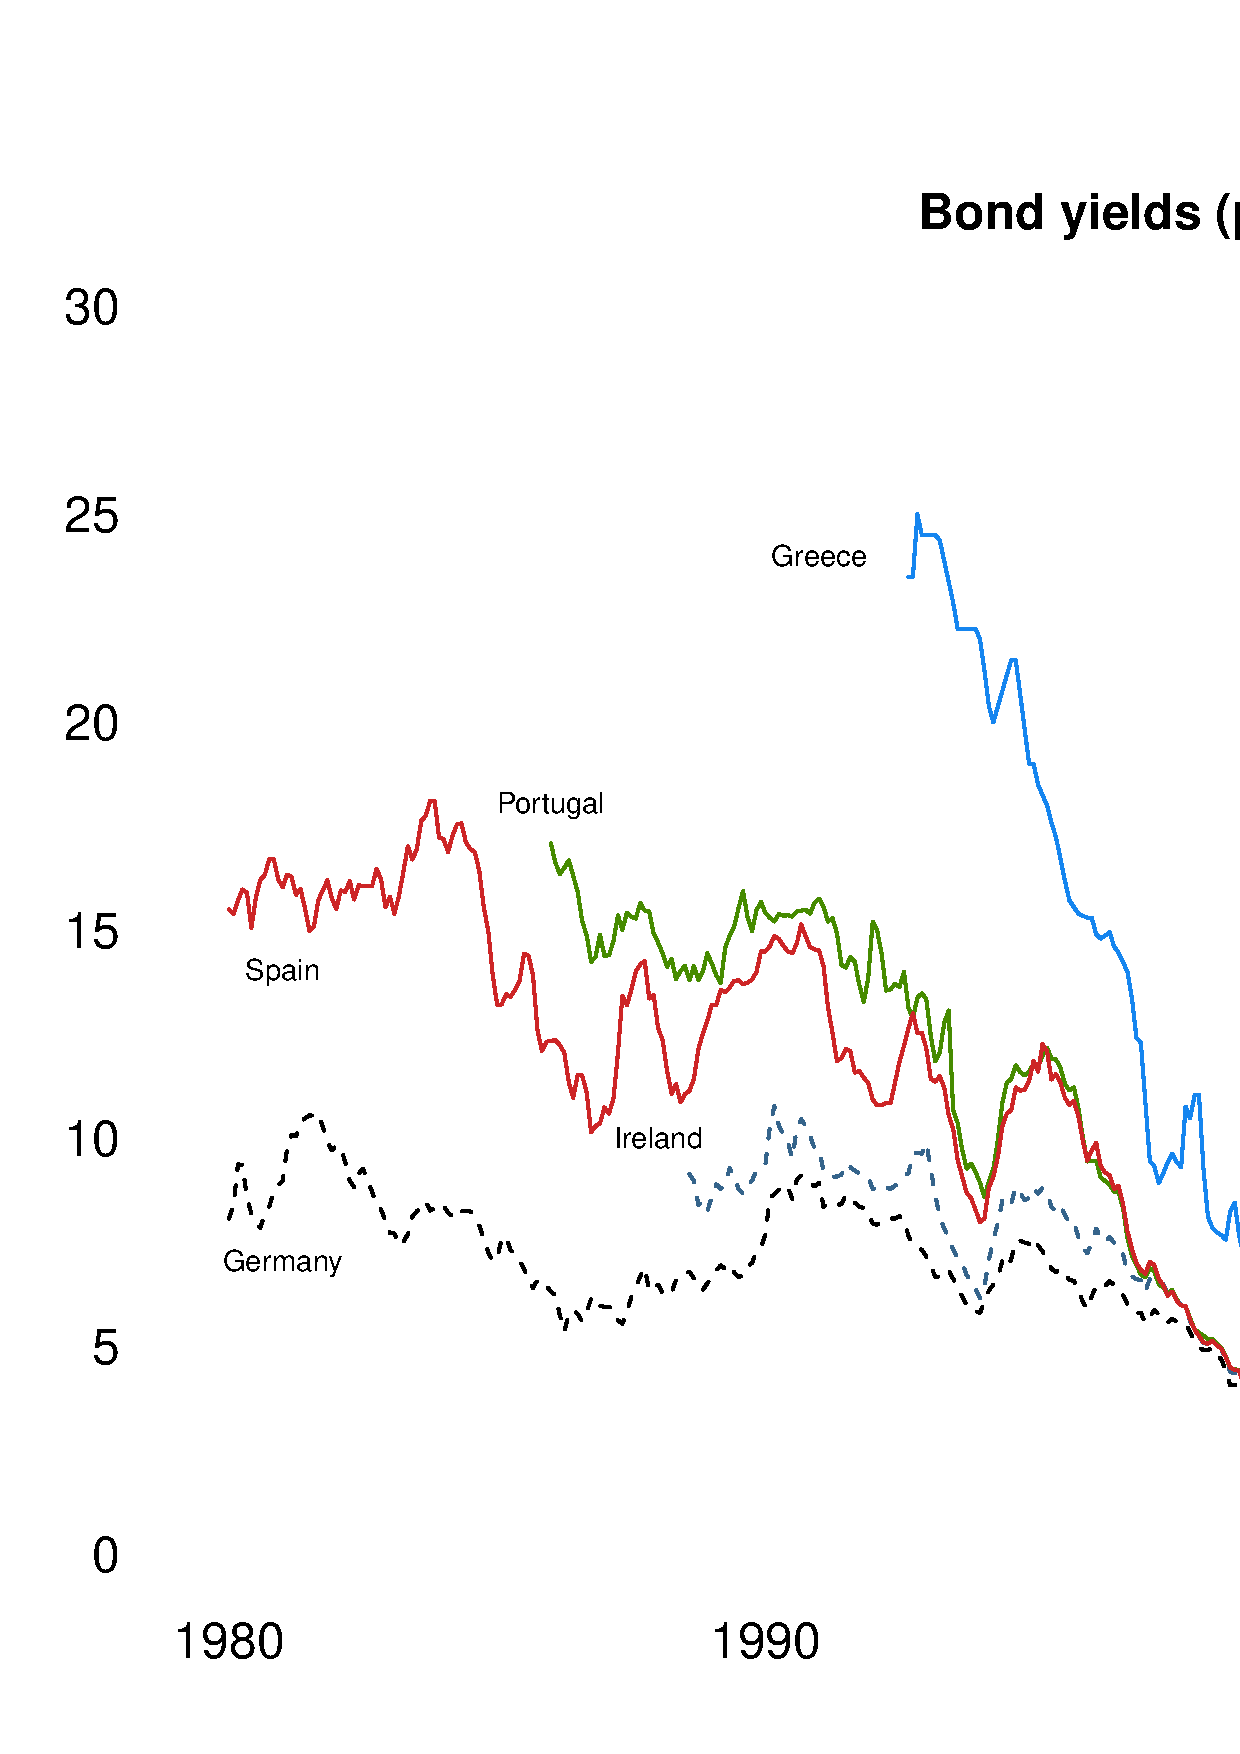
\includegraphics[scale=.3]{bond_yields.png}
    \caption{Government bond yields, 10 years' maturity. Data: Eurostat}
    \label{fig:bonds}
  \end{figure}
%------------------------------------------------

%--------------------------------------
\begin{figure}
  \includegraphics[scale=.3]{crisis_spain}
  \caption{Development of budget surplus and public debt in Spain. Data: Eurostat}
  \label{fig:spain}
\end{figure}
%--------------------------------------

%--------------------------------------
\begin{figure}
  \includegraphics[scale=.3]{within_eu_exports}
  \caption{Average share of EU exports to other member states for 2002-2016. Data: Eurostat}
  \label{fig:exports}
\end{figure}
%--------------------------------------

%--------------------------------------
\begin{figure} \centering
    \includegraphics[scale=.3]{debt_NYT.png}
    \caption{Debt among selected European economies. Source: New York Times} 
    \label{fig:inter_debt}
\end{figure}
%--------------------------------------
\clearpage
%------------------------------------------------------------------------------
% DEBT-DEFICIT
\subsection{Relation between deficit and debt.}
We've discussed repeatedly the development of deficit and debt over time in certain European countries. 
It is quite straightforward to see how debt is caused by deficits, but we haven't really discussed how the debt to GDP ratio relates to the deficit to GDP ratio. 
Let's say that, in nominal terms, the public debt at the end of a year $t$ is $B_t$ and the deficit is $D_t$. 
$D_t$ will equal
\begin{align}
  B_t-B_{t-1}=D_t
\end{align}

The convergence criteria set out by the Maastricht Treaty are based on ratios rather than levels, so using $b_t$ and $d_t$ to denote debt and deficit to GDP ratios respectively and $Y$ for GDP we can rewrite eq. 1 as
\begin{align}
  \frac{B_t-B_{t-1}}{Y_t} &= \frac{D_t}{Y_t}\\
  b_t-\frac{B_{t-1}}{Y_t} &= d_t
\end{align}

Note that the second term in eq.3 is
\begin{align}
  \frac{B_{t-1}}{Y_t} = \frac{B_{t-1}}{Y_{t-1}}\frac{Y_{t-1}}{Y_t} = \frac{b_{t-1}}{1+g_t}
\end{align}\marginnote{\begin{align*} g_t=\frac{Y_t-Y_{t-1}}{Y_t}=\frac{Y_t}{Y_{t-1}}-1 \end{align*}}

We can then rewrite eq.3 as
\begin{align}
  b_t-\frac{b_{t-1}}{1+g_t} &= d_t\\
  b_t-b_{t-1} &= (1+g_t)d_t-g_tb_t
\end{align}

For a constant debt-to-GDP ratio we need $b_t$ to equal $b_{t-1}$ which implies that the deficit-to-GDP ratio equals
\begin{align}
  (1+g_t)d_t-g_tb_t &=0 \\
  dt &= \frac{g_tb_t}{1+g_t} = \frac{g_t}{1+g_t}b_t
\end{align}

The Maastricht Treaty has set the convergence criteria to $b_t=60\%$ and $d_t=3\%$ so eq.8 would be satisfied when the growth rate is about 5\%.\footnote{Actually 5.3\%}.
The implicit assumption is that real GDP growth is 3\% and inflation is 2\%, equalling a nominal growth rate of 5\%. 
If a country is able to keep the debt level constant then naturally the debt-to-GDP ratio will decrease due to GDP growth. 
This also implies that the deficit becomes larger at high nominal growth rates. 

\clearpage
%------------------------------------------------------------------------------
% EU response
\section{Response by the EU}
One of the main obstacles in dealing with the eurocrisis is that what is essentially an economic problem required a solution with political backing. 
It became evident that there was a break down in confidence among member states and that different countries had very different preferences about how to solve the crisis.\marginnote{One of the shadiest thing to emerge was the fact that Goldman Sachs, a key player in the Great Recession, had helped the Greek government to hide some of its deficit in the books using currency swaps.} 
A main narrative was that the Southern eurozone members had been very reckless in their finance and that they only had themselves to blame really. 
Needless to say, governments from Northern eurozone countries were very reluctant to go ahead with some of the proposed solutions. 
A couple of solutions to the crisis that eventually didn't make it include
\begin{enumerate}
  \item Issue eurobonds
  \begin{itemize}
    \item Allowed governments to refinance debts as high-yield countries benefit from creditworthiness of low-yield countries
    \item Creates a moral hazard problem as it is possible subject to free riding
  \end{itemize}
  \item Fiscal transfers
  \begin{itemize}
    \item Basically rich eurozone countries compensating poor eurozone countries for their losses
    \item No system in place to do this, and would need political backing which is unlikely to be popular with population of richer countries
  \end{itemize}
  \item Kick Greece out of the euro\marginnote{An interesting development was the story that Finland had achieved a separate deal with Greece in settling the debt, where Greece used some of its islands as collateral.}
  \begin{itemize}
    \item Return to drachme, Greece would be able to set own monetary policy and regain competitiveness\footnote{Would still costs a lot of money to Greece because the debt has to be repaid.}
    \item Would create undesired precedent and risk stability of the whole euro project
  \end{itemize}
  \item Quantitative easing (QE)
  \begin{itemize}
    \item Can help boost economic activity
    \item Germany is not a fan of QE although the ECB did engage in some form of QE eventually
  \end{itemize}
\end{enumerate}

% Measures
The EU eventually did agree on the following measures aimed at helping member states that found themselves in financial difficulties
\begin{enumerate}
  \item European Financial Stability Facility (EFSF)
  \begin{itemize}
    \item June 2010
    \item Temporary crisis resolution mechanism for euro area member states
    \item Financed through the issuance of bonds and other debt instruments on the capital markets (capacity of \texteuro 500 billion)\footnote{Guaranteed by the other euro area member states so almost sort like eurobonds.}
    \item Assistance was used to provide loans, recapitalise banks, or buy sovereign debt    
    \item Provided assistance to Ireland, Portugal, Greece\footnote{The EFSF was superseded by the European Stability Mechanism. Although it doesn't provide assistance any more, it is still operational to \begin{itemize}
    \item Receive loan payments from beneficiary countries
    \item Make interest and principal payments to holders of EFSF bonds
    \item Roll over outstanding EFSF bonds, as the maturity of loans provided to Ireland, Portugal and Greece is longer than the maturity of bonds issued by the EFSF
  \end{itemize}}
  \end{itemize}
  \item European Financial Stabilisation Mechanism (EFSM)
  \begin{itemize}
    \item May 2010 (first bonds sold in January 2011)
    \item Provides financial assistance to any EU member state which is facing severe financial disturbances
    \item Country can get up to \texteuro 60 billion in assistance from the European Commission
    \item The fund is financed through  bond sales, using EU budget as collateral    
    \item Provided assistance to Ireland and Portugal, and a short term loan to Greece
  \end{itemize}
\end{enumerate}

% ESM
These more or less temporary measures were followed up by a more formalised structure to assist eurozone member states under the European Stability Mechanism (ESM).\footnote{Basically the EFSF expanded.}
The ESM was established in October 2012, and aimed to help overcome the problem for countries facing a debt crisis that they couldn't get credit from international financial markets or at unfavourable rates. 
The ESM, in combination with the running EFSF, has a budget of \texteuro 700 billion.
Between 2012-2016, the programme disbursed about \texteuro 250 billion to five countries
\begin{itemize}
  \item Ireland, February 2011 (part of EFSF)
  \item Portugal, June 2011 (part of EFSF)
  \item Greece, March 2012 (part of EFSF)
  \item Spain, October 2012
  \item Cyprus, May 2013
  \item Greece, August 2015 (still running)
\end{itemize}

Note that the ESM is just a temporary backstop, as acknowledged by the programme itself. 
It serves as a safety net, so that countries can cover the running costs, but does not address structural issues. 
Within the Maastricht Treaty there is actually a provision against these types of financial assistance as it could lead to lapses in fiscal discipline. 

%------------------------------------------------
\clearpage
% ECB response
\section{Response by the European Central Bank}
What did the European Central Bank, responsible for monetary policy in the eurozone, actually do?\footnote{Recall that the ECB is independent, in order to limit government interference in its policy.}
Given its original mandate, the ECB's preferred course of action is to do nothing at all, and let governments sort out the mess.
However, as the crisis progressed and got worse they had to come into action at some point. 
A main fear was the risk of contagion from smaller, peripheral economies, such as Greece and Portugal, to larger central ones such as Italy and possibly France.\footnote{Risk of contagion was a serious issue as for instance Italy owed France about 20\% of French GDP.} 
The ECB took two type of measures
\begin{enumerate}
  \item Standard
  \begin{itemize}
    \item Adjusting the key interest rates downwards
    \item Taken due to the macroeconomic circumstances and the risk for price stability
    \item Short-term interest rates are close to zero at the moment
  \end{itemize}
  \item Non-Standard
  \begin{itemize}
    \item Measures include fixed rate lending, providing longer maturity liquidity, expanding set of assets that can serve as collateral
    \item Taken because the banking system wasn't functioning properly
    \item ECB wanted to have a proper transmission of their monetary policy    
  \end{itemize}
\end{enumerate}

In addition to these measures the ECB took a number of unconventional steps to show the commitment of the bank to guaranteeing the stability of the Eurozone
\begin{itemize}
  \item Long Term Refinancing Operations (LTRO)
  \begin{itemize}
    \item ECB committed itself to refinancing operations for multiple years, rather than couple of months which is common    
    \item LTROs are provided at relatively cheap rates
    \item ECB serves as lender of first resort to troubled banks, these banks could then help struggling governments by purchasing debt    
  \end{itemize}
  \item Securities Market Program (SMP)
  \begin{itemize}
    \item Purchasing government and private debt, from countries facing problems
    \item Similar to QE, main difference is that ECB keeps the books balanced; offsetting the purchases by offering the banks interest-bearing deposits\footnote{Both the Federal Reserve and the Bank of England used quantitative easing (QE) which is just turning on the money press which injects liquidity in the system. In contrast, the ECB keeps the money supply stable to avoid fuelling inflation, by sterilising the purchases, offering deposits equal in value to the government bonds it holds.}
  \end{itemize}
  \item Outright Money Transactions (OMT)
  \begin{itemize}
    \item Follow up of SMP (in September 2012)
    \item Under certain circumstances a state could request the ECB to buy bonds     
    \item OMTs haven't been used yet as none of the candidate countries met the criteria\footnote{See web page on its \href{https://www.ecb.europa.eu/press/pr/date/2012/html/pr120906_1.en.html}{technical features}.}
  \end{itemize}
\end{itemize}

An important thing to note here is that when the ECB buys large quantities of bonds from a country that is at risk of default, the bank puts itself at risk. 
If the ECB gets into to much difficulty, the Germans have agreed to bail out the bank. 
Therefore, you can understand why the Germans are not very keen on the ECB buying large quantities of bonds.\footnote{Their top man at the bank,  J\"urgen Stark, actually resigned when the policy was implemented.}
Some people at the ECB are indeed not happy with this course of action as the original mandate of the bank is to target inflation, rather than sorting out the financial mess of the eurocrisis, the result mainly of countries not sticking to their budget requirements. 
Nonetheless, the ECB measures have been very important as they showed commitment to keeping the euro intact. 
Still, it doesn't address any of the core issues that were responsible for the crisis.  
To guarantee long run stability, a political solution must be implemented to overcome the remaining economic obstacles. 

%------------------------------------------------------------------------------
% INFLATION DIFFERENCES
\subsection{Inflation differences}
The optimum currency area emphasised the risk of asymmetric shocks, and certainly the effects of the Great Recession has had very divergent effects across the Eurozone. 
One issue here is the inflation rate where countries such as Greece and Italy have had persistently higher inflation rates compared to for instance Germany. 
The problem with a common currency is that a country with high inflation rates will see a loss in competitiveness as the real exchange rate appreciates. 
As illustration, consider the price of a good in Italy which has price $P$ and the same good has price $P^*$ in Germany. 
Prior to the introduction of the Euro we could compare the price using exchange rate $E$, and we could construct a real exchange rate as $\frac{EP}{P^*}$
Now with the introduction of the euro $E$ is fixed, so inflation will cause $\frac{P}{P^*}$ to increase and an appreciation in $\frac{EP}{P^*}$ leading to a loss in competitiveness. 
Some explanations for the divergence in inflation rates include\footnote{Additionally, inflation is low in countries that had a current account surplus and high in countries with a current account deficit.}
\begin{itemize}
  \item Balassa-Samuelson effect
  \begin{itemize}
    \item \textit{"Equilibrium real exchange rates of countries that enjoy lasting fast growth, because they are catching up from low development levels, follow an appreciating trend"}
    \item i.e. inflation rates sign of increase in competitiveness 
  \end{itemize}
  \item ECU fixed at wrong rates\footnote{Likely that the German Deutschmark was undervalued and the Greek Drachme overvalued.}
  \item Autonomous wage and price setting
  \begin{itemize}
    \item Wage increases caused by factors other than labour productivity decreases competitiveness
    \item e.g. raising minimum wage, bargaining by sectors that don't face much competition such as civil servants, administered prices in transport and energy
  \end{itemize}
  \item Mistakes in policy
  \begin{itemize}
    \item Government could increase prices and wages through for instance expansionary fiscal policies
  \end{itemize}  
  \item Different preferences
  \begin{itemize}
    \item A country poor at collecting taxes might prefer inflation tax or seigniorage
    \item Variation in consumption baskets can cause different inflations across countries with same monetary policy
  \end{itemize}
\end{itemize}
\clearpage

%------------------------------------------------------------------------------
% SINCE CRISIS
\section{Development since crisis}
The process of economic and monetary integration in the EU is all about convergence of economic performance; raising living standards. 
For a time this process seemed to have paid off during the boom years in the first decade of the 21st century, but it unravelled quickly in the years after the crisis. 
Again focusing on a number of macroeconomic indicators we can illustrate how the crisis led to a divided Europe. 

\begin{enumerate}
  \item Growth (figure~\ref{fig:growth_2007})
  \begin{itemize}
    \item As a whole, the Eurozone only managed to exceed its 2007 level round about 2014
    \item Germany got over the recession relatively quick
    \item The UK experienced slower recovery
    \item Spain is only catching up now, and Italy is still lagging
  \end{itemize}

  \item Investment (figure~\ref{fig:capital_2007})
  \begin{itemize}
    \item Investment levels in the Eurozone are still low
    \item Germany and France only recently caught up with their 2007 level
    \item Eurozone as a whole still lagging, again Italy and Spain are far behind
  \end{itemize}


  \item Unemployment (figure~\ref{fig:unemployment_2007})
  \begin{itemize}
    \item There is a huge difference in unemployment rates between the North and South of the Eurozone
    \item Eurozone average at about 10\% is relatively high, but decreasing
    \item Mediterranean countries show no strong decreasing trend
    \item Moreover, youth unemployment is very high in the Southern countries
  \end{itemize}

  \item Exports (figure~\ref{fig:exports_1999})
  \begin{itemize}
    \item Can countries export their way back to prosperity?
    \item Ireland is doing well, but that came at the cost of reducing wages
    \item The Mediterranean countries still have low export levels
    \item Noticeable is Italy which is one of the largest economies in the world and part of the G7
  \end{itemize}
\end{enumerate}


%--------------------------------------
\begin{figure}
  \includegraphics[scale=.3]{growth_since_2007}
  \caption{Growth for large European economies (2007=100). Data: Eurostat}
  \label{fig:growth_2007}
\end{figure}
%--------------------------------------

%--------------------------------------
\begin{figure}
  \includegraphics[scale=.3]{capital_formation_since_2007}
  \caption{Capital formation in large European economies (2007=100). Data: Eurostat}
  \label{fig:capital_2007}
\end{figure}
%--------------------------------------

\clearpage

%--------------------------------------
\begin{figure}
  \includegraphics[scale=.3]{unemployment_since_2007}
  \caption{Unemployment since 2007 for the Eurozone as a whole and Mediterranean countries (Greece, Italy, Spain, Portugal) and some countries in the Rhine basin (Austria, Germany, the Netherlands). Data: Eurostat}
  \label{fig:unemployment_2007}
\end{figure}
%--------------------------------------
%--------------------------------------
\begin{figure}
  \includegraphics[scale=.3]{exports_since_1999}
  \caption{Exports since 1999 (=100). Data: Eurostat}
  \label{fig:exports_1999}
\end{figure}
%--------------------------------------

%------------------------------------------------------------------------------
\clearpage
% GREEK DEPRESSION
\section{The Greek Depression}
Greece became ground zero for the European debt crisis after it emerged in late 2009 that is had been understating its debt figures for years.\footnote{They misreported their numbers at Eurostat which the EU uses.}Rather unsurprisingly this led to serious doubts about the state of the Greek economy and government finances in particular leading to high yields on its bonds, effectively barring the country from lending money on the international market.  
Figure~\ref{fig:greece} shows the development of Greece's GDP over time. 
Although the country experienced a substantial period of growth from 1995 onwards, the crisis destroyed much of the progress made over the years with current GDP being at the level of 2000.
Figure~\ref{fig:contraction} illustrates just how severe the contraction of the Greek economy has been, wiping away about 25\% of GDP.
%------------------------------------------------
\begin{figure} \centering
    \includegraphics[scale=.3]{greece_gdp.png}
    \caption{GDP, unadjusted and seasonally and calendar adjusted, for Greece over time. Greece GDP (unadjusted and adjusted) Data source: Eurostat}
    \label{fig:greece}
\end{figure}
%------------------------------------------------ 
%------------------------------------------------
\begin{figure} \centering
    \includegraphics[scale=.3]{greece_contraction.png}
    \caption{Contraction of the Greek economy since the second quarter of 2007. Arguably, the situation in Greece has been worse than that in America during the Great Depression, and possibly comparable to the German situation during the Weimar Republic. Data: Eurostat}
    \label{fig:contraction}
\end{figure}
%------------------------------------------------

Unable to repay or refinance its debt Greece was on the brink of bankruptcy in the Spring of 2010 and needed international assistance to stay afloat.\footnote{These were bail outs provided by the Troika of the European Commission, the European Central Bank, and the International Monetary Fund.}
To give a chronological overview of the events in Greece related to the debt crisis:
\begin{itemize}
  \item 2009
  \begin{itemize}
    \item October: budget deficit expected to reach 12.5\% of GDP
    \item October-December: Credit status downgraded     
  \end{itemize}
  \item 2010
  \begin{itemize}
    \item February: first austerity package
    \item March: second austerity package
    \item April: first bail out request
    \item May: Bail out agreed and third austerity package\marginnote{The implementation of the austerity measures are followed by civil unrest.}
  \end{itemize}
  \item 2011
  \begin{itemize}
    \item June: fourth austerity package
    \item October: fifth austerity package, debt haircut of 50\% agreed with international lenders\footnote{Half of Greece's public debt was reduced up to 75\%. This was repackaged as a new loan. Investors were willing to accept this large immediate loss over future uncertainty and possible larger losses. The two largest Cypriot banks were among the losers as they had a lot of assets in Greek bonds, and a year later they collapsed.}
  \end{itemize}
  \item 2012
  \begin{itemize}
    \item January: sixth austerity package
    \item February: second bail out\footnote{Political deadlock after elections from May till June.}
    \item November: Seventh austerity package
  \end{itemize}  
  \item 2015
  \begin{itemize}
    \item January: Elections won by current PM
    \item February: 4-month extension on loan brokered between Greece and other Eurozone members
    \item June-July: Referendum held on another bailout agreement, rejected by population
    \item July: Additional Greek request for financial aid rejected, Greece defaults on IMF loan
  \end{itemize}  
\end{itemize}


The assistance that the Greeks received came with some strings attached though. 
\begin{itemize}
  \item Harsh austerity terms (figure~\ref{fig:austerity})
  \begin{itemize}
    \item Cuts in public spending such as investments (figure~\ref{fig:finance})
    \item Tax increases    
  \end{itemize}
  \item Government overhaul
  \begin{itemize}
    \item Reducing size of the government apparatus
    \item Cutting back on pensions
    \item Importantly there were no cuts to defense spending in terms of percentage GDP    
  \end{itemize}
  \item Ending tax evasion by its citizens\footnote{Note also that the shipping industry in Greece pays very little tax. }
  \item Making business in Greece easier
\end{itemize}

%------------------------------------------------
\begin{figure} \centering{}
    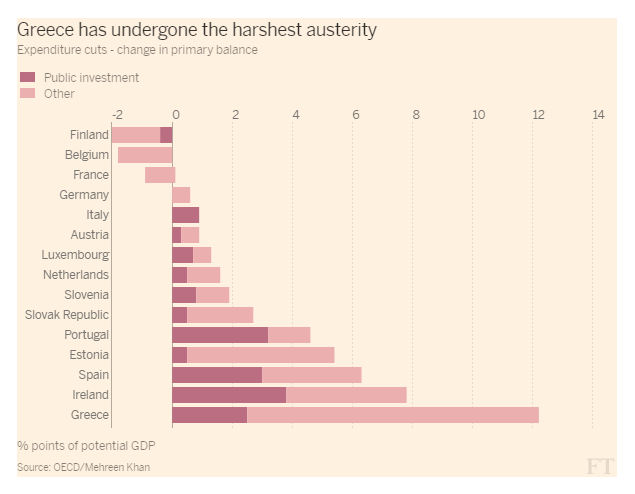
\includegraphics[scale=.3]{austerity}
    \caption{Austerity across Europe. Source: Financial Times}
    \label{fig:austerity}
\end{figure}
%------------------------------------------------

%------------------------------------------------
\begin{figure} \centering
    \includegraphics[scale=.3]{greece_finances.png}
    \caption{Public spending and tax revenues as a percentage of GDP in Greece. Data source: Eurostat}
    \label{fig:finance}
\end{figure}
%------------------------------------------------ 

The outside intervention entailed a serious loss of Greek autonomy across a number of areas, specifically government spending, which made a lot of people very angry. 
Over the years, between 2010-2015 Greece has received three bail outs amounting to a total of 
\texteuro 240 billion, or about \texteuro 22,000 per capita. 
It is important to note that most of this bail out money went either to paying off existing debts or recapitalising the banks, and did not benefit directly the population.\footnote{I.e. the bail outs were not used for investments in infrastructure, education, or something similar.}
A lot of structural problems in Greece still need to be addressed while public debt is at a record high. 
There are some early signs of improvement where the Greek economy is even reporting some positive growth rates, but the process of getting the economy to be competitive again is a long and painful one. 
For instance it involves reduction in wages as shown in figure~\ref{fig:labour_costs}.%------------------------------------------------
\begin{figure} \centering
    \includegraphics[scale=.3]{greece_labour_costs.png}
    \caption{Unit labour costs in Greece and the Eurozone (dashed line) Data source: OECD}
    \label{fig:labour_costs}
\end{figure}
%------------------------------------------------  

%------------------------------------------------------------------------------
\clearpage
\subsection{Background: How does a sovereign default happen?}
Normally sovereign defaults are pretty rare as most developed economies are relatively stable. 
Now image that the market perceives that a particular country has a 10\% chance of a default over the next year, leading to a 50\% default on its outstanding debt. 
In this scenario the country has to pay a 5\% premium on debt relative to safe assets.\marginnote{Safe assets here is debt with virtually no default risk.} 
The extra premium will place an additional burden on the government, this could lead to a situation where the interest costs rise above the funds that country can access to pay off the interest payments.\marginnote{Alternatively the country's GDP could expand in order to keep debt stable.} 
Subsequently, the market for government bonds might cease to operate as the country is deemed not credit-worthy, which means an increase in the risk of default going from unlikely to likely. 
It is important to note that the closing of a bond market is an rare and abrupt events. 
People often don't see it coming. 
After a default a country needs to restructure it debt which often involves writing off part of it, in order to restore the debt level to a more sustainable level.



%------------------------------------------------------------------------------
\end{document}
